\chapter{Experiments}\label{sec:experiments}

The experiments chapter walks through the goals, trials, and conclusions from each experiment, following a systematic evaluation of relay strategies across diverse configurations.

\section{Channel Model Validation}\label{sec:channel-model-validation}

The detailed experimental validation of the channel models, including comparison against closed-form theoretical BER expressions (AWGN, Rayleigh, Rician, and MIMO configurations), is provided in \textbf{Appendix~\ref{chap:app-validation}}.

\section{SISO BPSK Performance (Baseline Relay Comparison)}\label{sec:siso-bpsk-performance-baseline-relay-comparison}

\textbf{Goal:} Evaluate baseline classical and AI-based relay strategies on single-antenna configurations across different fading environments.

\textbf{Trials:} - \textbf{Topology:} SISO - \textbf{Modulation scheme:} BPSK - \textbf{Channel:} AWGN, Rayleigh, Rician (K=3) - \textbf{Equalizers:} None - \textbf{NN architecture:} Supervised (MLP, Hybrid), Generative (VAE, CGAN), Sequence (Transformer, Mamba S6, Mamba-2 SSD) - \textbf{NN activation:} tanh

\textbf{Conclusion:} AI relays selectively outperform AF and, on selected channels (AWGN, Rician), DF at low SNR (0--4 dB). However, under Rayleigh fading, classical DF dominates even at low SNR. Across all channels, classical DF remains dominant at medium-to-high SNR (\(\geq 6\) dB), matching or exceeding all AI methods with zero parameters.

\subsection{Results Tables}\label{sec:results-tables}

\textit{[Detailed tabular results have been moved to Appendix~\ref{chap:app-tables}]}


\textit{[Detailed tabular results have been moved to Appendix~\ref{chap:app-tables}]}


\textit{[Detailed tabular results have been moved to Appendix~\ref{chap:app-tables}]}


\subsection{Results Figures}\label{sec:results-figures-1}

\begin{figure}[H]
\centering
\centering
\pandocbounded{
\includegraphics[width=\linewidth,height=0.45\textheight,keepaspectratio]{results/awgn_comparison_ci.png}}
\caption{AWGN channel --- BER vs.~SNR for all nine relay strategies with 95\% CI. AI relays outperform classical methods at low SNR; DF dominates at medium-to-high SNR.}\label{fig:fig9}
\end{figure}

\begin{figure}[H]
\centering
\centering
\pandocbounded{
\includegraphics[width=\linewidth,height=0.45\textheight,keepaspectratio]{results/fading_comparison.png}}
\caption{Rayleigh fading --- BER vs.~SNR for all nine relay strategies with 95\% CI.}\label{fig:fig10}
\end{figure}

\begin{figure}[H]
\centering
\centering
\pandocbounded{
\includegraphics[width=\linewidth,height=0.45\textheight,keepaspectratio]{results/rician_comparison_ci.png}}
\caption{Rician fading (K=3) --- BER vs.~SNR for all nine relay strategies with 95\% CI.}\label{fig:fig11}
\end{figure}

\section{MIMO 2x2 BPSK Performance}\label{sec:mimo-2x2-bpsk-performance}

\textbf{Goal:} Evaluate relay strategies under spatial multiplexing and various interference cancellation techniques.

\textbf{Trials:} - \textbf{Topology:} MIMO 2x2 - \textbf{Modulation scheme:} BPSK - \textbf{Channel:} Rayleigh - \textbf{Equalizers (in MIMO only):} ZF, MMSE, SIC - \textbf{NN architecture:} Supervised (MLP, Hybrid), Generative (VAE, CGAN), Sequence (Transformer, Mamba S6, Mamba-2 SSD) - \textbf{NN activation:} tanh

\textbf{Conclusion:} The MIMO equalization hierarchy (ZF \textless{} MMSE \textless{} SIC) holds for all relay types. The AI advantage at low SNR is preserved under ZF and MMSE (where Mamba S6 achieves the lowest BER), but under the superior SIC equalization, classical DF provides the lowest BER at all low-to-medium SNR points. Relay processing gains and MIMO equalization gains are additive.

\subsection{Results Tables}\label{sec:results-tables-1}

\textit{[Detailed tabular results have been moved to Appendix~\ref{chap:app-tables}]}


\textit{[Detailed tabular results have been moved to Appendix~\ref{chap:app-tables}]}


\textit{[Detailed tabular results have been moved to Appendix~\ref{chap:app-tables}]}


\subsection{Results Figures}\label{sec:results-figures-2}

\begin{figure}[H]
\centering
\centering
\pandocbounded{
\includegraphics[width=\linewidth,height=0.45\textheight,keepaspectratio]{results/mimo_2x2_comparison_ci.png}}
\caption{2×2 MIMO with ZF equalization --- BER vs.~SNR for all nine relay strategies with 95\% CI.}\label{fig:fig12}
\end{figure}

\begin{figure}[H]
\centering
\centering
\pandocbounded{
\includegraphics[width=\linewidth,height=0.45\textheight,keepaspectratio]{results/mimo_2x2_mmse_comparison_ci.png}}
\caption{2×2 MIMO with MMSE equalization --- BER vs.~SNR for all nine relay strategies with 95\% CI.}\label{fig:fig13}
\end{figure}

\begin{figure}[H]
\centering
\centering
\pandocbounded{
\includegraphics[width=\linewidth,height=0.45\textheight,keepaspectratio]{results/mimo_2x2_sic_comparison_ci.png}}
\caption{2×2 MIMO with MMSE-SIC equalization --- BER vs.~SNR for all nine relay strategies with 95\% CI.}\label{fig:fig14}
\end{figure}

\section{Parameter Normalization \& Complexity Trade-off}\label{sec:parameter-normalization-complexity-trade-off}

\textbf{Goal:} Isolate architectural inductive biases from parameter count effects and characterize the complexity-performance trade-off for relay denoising.

\textbf{Trials:} - \textbf{Topology:} SISO, MIMO 2x2 - \textbf{Modulation scheme:} BPSK - \textbf{Channel:} AWGN, Rayleigh, Rician, MIMO (ZF, MMSE, SIC) - \textbf{Equalizers (in MIMO only):} None, ZF, MMSE, SIC - \textbf{NN architecture:} All normalized to \textasciitilde3,000 parameters, plus original sizes (169 to 26K) - \textbf{NN activation:} tanh

\textbf{Conclusion:} The relay denoising task exhibits an inverted-U complexity relationship: a minimal 169-parameter MLP matches models 140x larger, while excessive parameters (11K+) lead to overfitting. At a normalized scale of 3,000 parameters, the performance gap between feedforward and sequence architectures narrows to \textasciitilde1\% BER, indicating that parameter count rather than architectural choice is the primary performance driver. Generative VAE is a consistent underperformer due to probabilistic overhead.

\subsection{Results Tables}\label{sec:results-tables-2}

\textit{[Detailed tabular results have been moved to Appendix~\ref{chap:app-tables}]}


\textit{[Detailed tabular results have been moved to Appendix~\ref{chap:app-tables}]}


\textit{[Detailed tabular results have been moved to Appendix~\ref{chap:app-tables}]}


\textit{[Detailed tabular results have been moved to Appendix~\ref{chap:app-tables}]}


\textit{[Detailed tabular results have been moved to Appendix~\ref{chap:app-tables}]}


\textit{[Detailed tabular results have been moved to Appendix~\ref{chap:app-tables}]}


\textit{[Detailed tabular results have been moved to Appendix~\ref{chap:app-tables}]}


\subsection{Results Figures}\label{sec:results-figures-3}

\begin{figure}[H]
\centering
\centering
\pandocbounded{
\includegraphics[width=\linewidth,height=0.45\textheight,keepaspectratio]{results/normalized_3k_all_channels.png}}
\caption{Normalized 3K-parameter comparison across all channels. At equal parameter budgets, all architectures converge to similar BER, with VAE being the consistent underperformer.}\label{fig:fig15}
\end{figure}

\begin{figure}[H]
\centering
\centering
\pandocbounded{
\includegraphics[width=\linewidth,height=0.45\textheight,keepaspectratio]{results/normalized_3k_awgn.png}}
\caption{Normalized 3K-parameter BER comparison on AWGN. Mamba-3K and Transformer-3K produce nearly identical BER, eliminating the gap seen at original parameter counts.}\label{fig:fig16}
\end{figure}

\begin{figure}[H]
\centering
\centering
\pandocbounded{
\includegraphics[width=\linewidth,height=0.45\textheight,keepaspectratio]{results/normalized_3k_rayleigh.png}}
\caption{Normalized 3K-parameter BER comparison on Rayleigh fading.}\label{fig:fig17}
\end{figure}

\begin{figure}[H]
\centering
\centering
\pandocbounded{
\includegraphics[width=\linewidth,height=0.45\textheight,keepaspectratio]{results/normalized_3k_rician_k3.png}}
\caption{Normalized 3K-parameter BER comparison on Rician fading (K=3).}\label{fig:fig18}
\end{figure}

\begin{figure}[H]
\centering
\centering
\pandocbounded{
\includegraphics[width=\linewidth,height=0.45\textheight,keepaspectratio]{results/complexity_comparison_all_relays.png}}
\caption{Complexity--performance trade-off. Training time vs.~parameter count vs.~BER improvement over DF at low SNR. The Minimal MLP (169 params) achieves the best efficiency.}\label{fig:fig19}
\end{figure}

\begin{figure}[H]
\centering
\centering
\pandocbounded{
\includegraphics[width=\linewidth,height=0.45\textheight,keepaspectratio]{results/master_ber_comparison.png}}
\caption{Master BER comparison --- consolidated view of all nine relay strategies across all six channel/topology configurations.}\label{fig:fig20}
\end{figure}

\section{Higher-Order Modulation Scalability (Constellation-Aware Training)}\label{sec:higher-order-modulation-scalability-constellation-aware-training}

\textbf{Goal:} Evaluate the generalizability of BPSK-trained relays to complex constellations and resolve the multi-level amplitude bottleneck.

\textbf{Trials:} - \textbf{Topology:} SISO - \textbf{Modulation scheme:} QPSK, 16-QAM - \textbf{Channel:} AWGN, Rayleigh - \textbf{Equalizers:} None - \textbf{NN architecture:} Supervised (MLP, Hybrid), Generative (VAE, CGAN), Sequence (Transformer, Mamba S6, Mamba-2 SSD) - \textbf{NN activation:} tanh, linear, clipped tanh (hardtanh), scaled tanh, scaled sigmoid - \textbf{Special case:} Constellation Aware training

\textbf{Conclusion:} QPSK performance mirrors BPSK perfectly due to I/Q independence. On 16-QAM, standard tanh compression causes a severe, irreducible BER floor (\textasciitilde0.22 at 16 dB). Replacing tanh with constellation-aware bounded activations (hardtanh, scaled tanh) bounded to the precise signal amplitude (\(3/\sqrt{10}\)) and retraining eliminates this floor. Sequence models benefit most, reducing their BER floor by 5x, though a gap to classical DF persists due to per-axis error accumulation.

\subsection{Results Tables}\label{sec:results-tables-3}

\textit{[Detailed tabular results have been moved to Appendix~\ref{chap:app-tables}]}


Table~\ref{tbl:table15} shows the BER at 16 dB for all relays across the three activation variants and both channel types.

\textit{[Detailed tabular results have been moved to Appendix~\ref{chap:app-tables}]}


Table~\ref{tbl:table16} summarises the 16-QAM and 20dB AWGN improvements for the sequence models.

\textit{[Detailed tabular results have been moved to Appendix~\ref{chap:app-tables}]}


\subsection{Results Figures}\label{sec:results-figures-4}

\begin{figure}[H]
\centering
\centering
\pandocbounded{
\includegraphics[width=\linewidth,height=0.45\textheight,keepaspectratio]{results/modulation/bpsk_awgn_ci.png}}
\caption{BPSK on AWGN --- all relay strategies with 95\% CI (baseline for modulation comparison).}\label{fig:fig21}
\end{figure}

\begin{figure}[H]
\centering
\centering
\pandocbounded{
\includegraphics[width=\linewidth,height=0.45\textheight,keepaspectratio]{results/modulation/bpsk_rayleigh_ci.png}}
\caption{BPSK on Rayleigh fading --- all relay strategies with 95\% CI.}\label{fig:fig22}
\end{figure}

\begin{figure}[H]
\centering
\centering
\pandocbounded{
\includegraphics[width=\linewidth,height=0.45\textheight,keepaspectratio]{results/modulation/qpsk_awgn_ci.png}}
\caption{QPSK on AWGN --- BER curves closely match the BPSK baseline (Figure~\ref{fig:fig21}), confirming I/Q splitting validity.}\label{fig:fig23}
\end{figure}

\begin{figure}[H]
\centering
\centering
\pandocbounded{
\includegraphics[width=\linewidth,height=0.45\textheight,keepaspectratio]{results/modulation/qpsk_rayleigh_ci.png}}
\caption{QPSK on Rayleigh fading --- same relative ordering as BPSK, confirming hypothesis generalisability.}\label{fig:fig24}
\end{figure}

\begin{figure}[H]
\centering
\centering
\pandocbounded{
\includegraphics[width=\linewidth,height=0.45\textheight,keepaspectratio]{results/modulation/qam16__awgn_ci.png}}
\caption{16-QAM on AWGN --- AI relays hit a BER floor near 0.22 at medium-high SNR due to \(\tanh\) compression of multi-level signals; AF outperforms DF at low SNR (Y}\label{fig:fig25}
\end{figure}

\begin{figure}[H]
\centering
\centering
\pandocbounded{
\includegraphics[width=\linewidth,height=0.45\textheight,keepaspectratio]{results/modulation/qam16__rayleigh_ci.png}}
\caption{16-QAM on Rayleigh fading --- wider BER gap between modulations under fading; all AI relays significantly worse than DF at every SNR point (N}\label{fig:fig26}
\end{figure}

\begin{figure}[H]
\centering
\centering
\pandocbounded{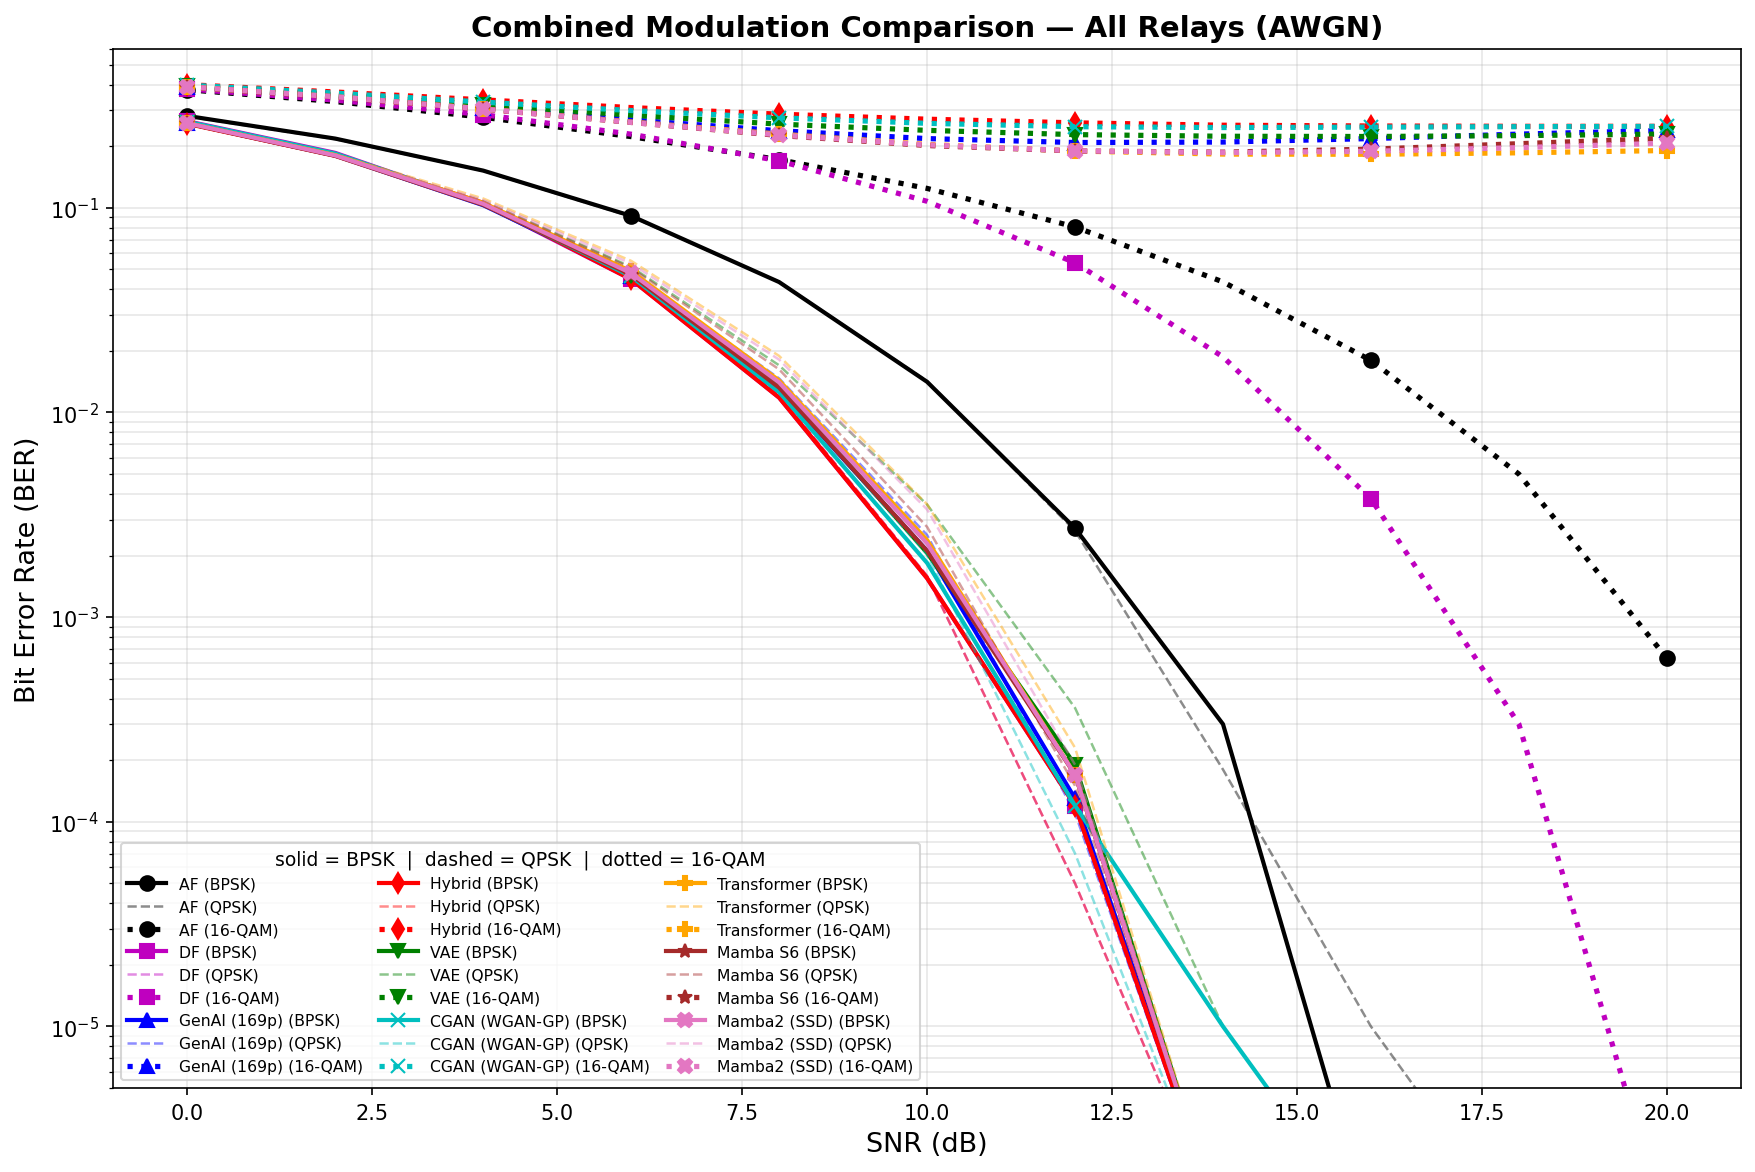
\includegraphics[width=\linewidth,height=0.45\textheight,keepaspectratio]{results/modulation/combined_modulation_awgn.png}}
\caption{Combined modulation comparison (AWGN) --- all nine relays across BPSK (solid), QPSK (dashed, overlapping BPSK), and 16-QAM (dotted). The BPSK/QPSK overlap confirms I/Q splitting equivalence. The 16-QAM dotted curves reveal the AI relay BER floor: all AI relays plateau near 0.18--0.25 while DF and AF continue decreasing.}\label{fig:fig27}
\end{figure}

\begin{figure}[H]
\centering
\centering
\pandocbounded{
\includegraphics[width=\linewidth,height=0.45\textheight,keepaspectratio]{results/qam16_activation/qam16_activation_awgn.png}}
\caption{16-QAM activation experiment (AWGN) --- dashed lines = tanh/BPSK baseline, solid = linear/QAM16, dotted = hardtanh/QAM16. Replacing tanh and retraining on QAM16 eliminates the BER floor for all AI relays except Hybrid. Sequence models (Transformer, Mamba S6, Mamba-2) benefit most, narrowing the gap to DF from \textasciitilde56× to \textasciitilde10×.}\label{fig:fig28}
\end{figure}

\begin{figure}[H]
\centering
\centering
\pandocbounded{
\includegraphics[width=\linewidth,height=0.45\textheight,keepaspectratio]{results/qam16_activation/qam16_activation_rayleigh.png}}
\caption{16-QAM activation experiment (Rayleigh fading) --- same trend under fading. The improvement is significant but the gap to DF/AF remains larger than on AWGN, consistent with fading amplifying modulation-order differences (Finding 6).}\label{fig:fig29}
\end{figure}

\begin{figure}[H]
\centering
\centering
\pandocbounded{
\includegraphics[width=\linewidth,height=0.45\textheight,keepaspectratio]{results/activation_comparison/bpsk_activation_awgn.png}}
\caption{BPSK constellation-aware activation comparison (AWGN). With \(A_{\max} = 1.0\), scaled tanh reduces to standard tanh. All three bounded activations achieve equivalent BER, confirming that BPSK is insensitive to activation choice.}\label{fig:fig30}
\end{figure}

\begin{figure}[H]
\centering
\centering
\pandocbounded{
\includegraphics[width=\linewidth,height=0.45\textheight,keepaspectratio]{results/activation_comparison/bpsk_activation_rayleigh.png}}
\caption{BPSK constellation-aware activation comparison (Rayleigh fading). Same pattern under fading --- activation choice has negligible effect on BPSK BER.}\label{fig:fig31}
\end{figure}

\begin{figure}[H]
\centering
\centering
\pandocbounded{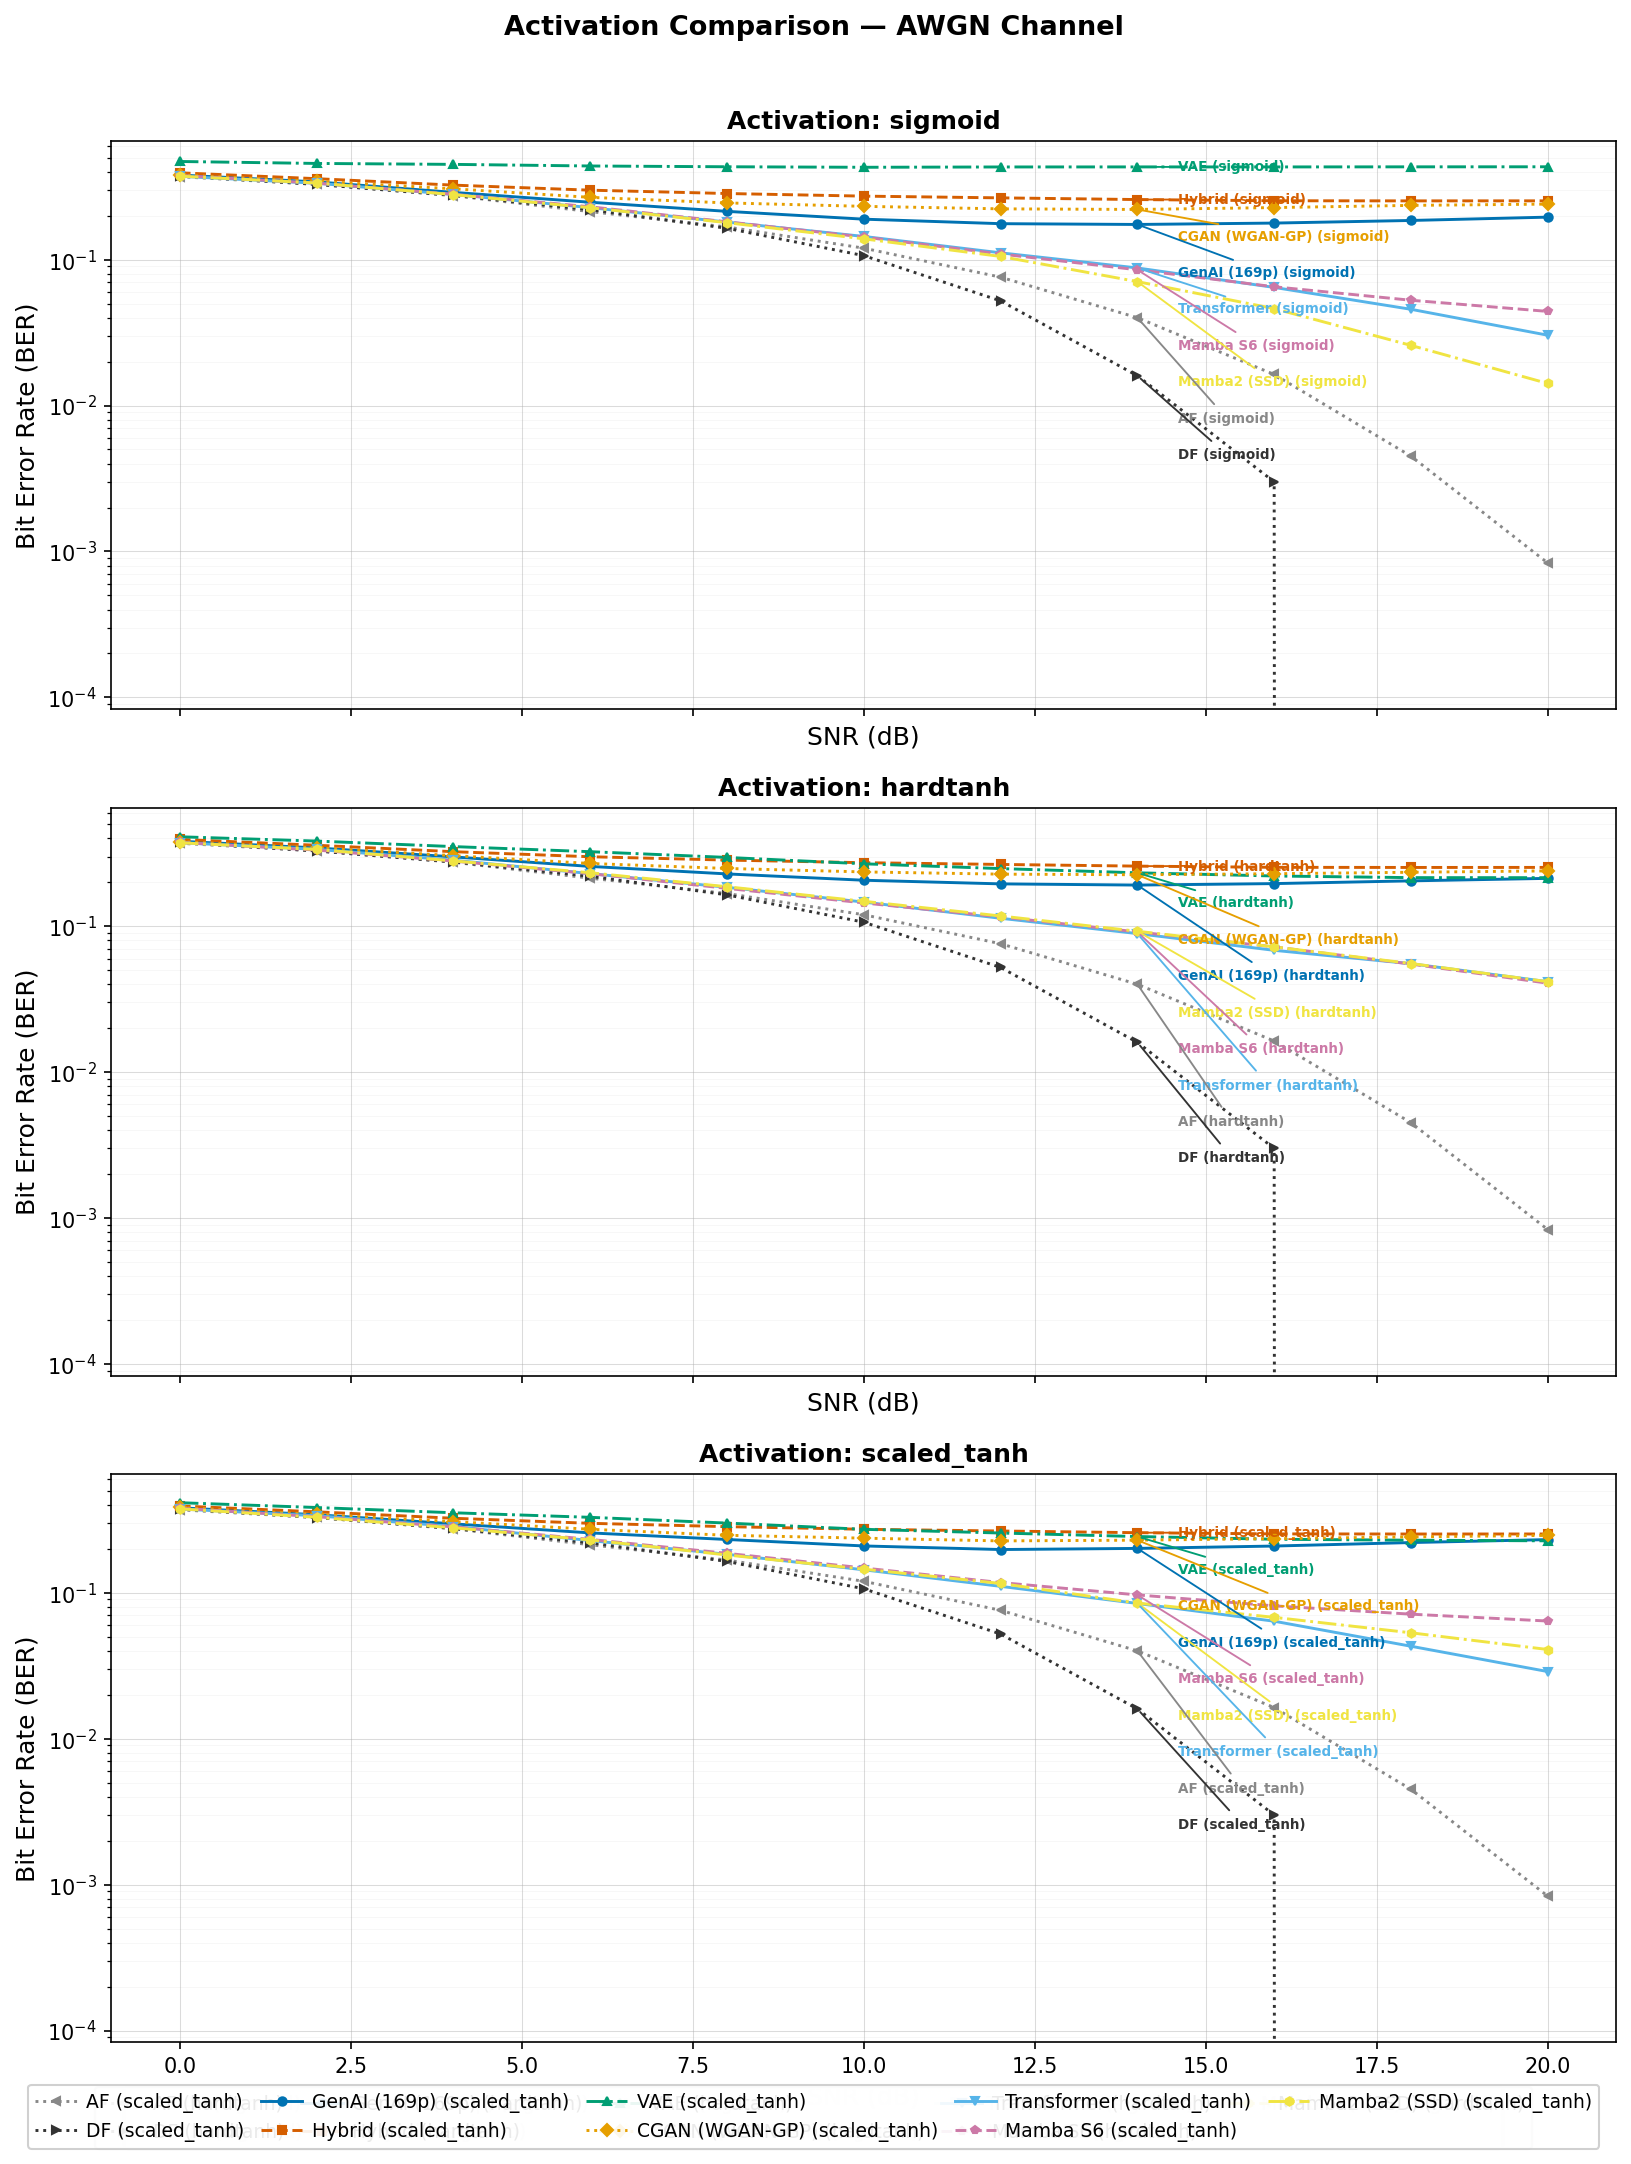
\includegraphics[width=\linewidth,height=0.45\textheight,keepaspectratio]{results/activation_comparison/qpsk_activation_awgn.png}}
\caption{QPSK constellation-aware activation comparison (AWGN). With \(A_{\max} = 0.7071\), the tighter clip range matches the binary I/Q components exactly. Sigmoid provides marginally lower BER for the Transformer relay at low SNR.}\label{fig:fig32}
\end{figure}

\begin{figure}[H]
\centering
\centering
\pandocbounded{
\includegraphics[width=\linewidth,height=0.45\textheight,keepaspectratio]{results/activation_comparison/qpsk_activation_rayleigh.png}}
\caption{QPSK constellation-aware activation comparison (Rayleigh fading). Similar trends under fading. The three activations remain closely matched for most relays.}\label{fig:fig33}
\end{figure}

\begin{figure}[H]
\centering
\centering
\pandocbounded{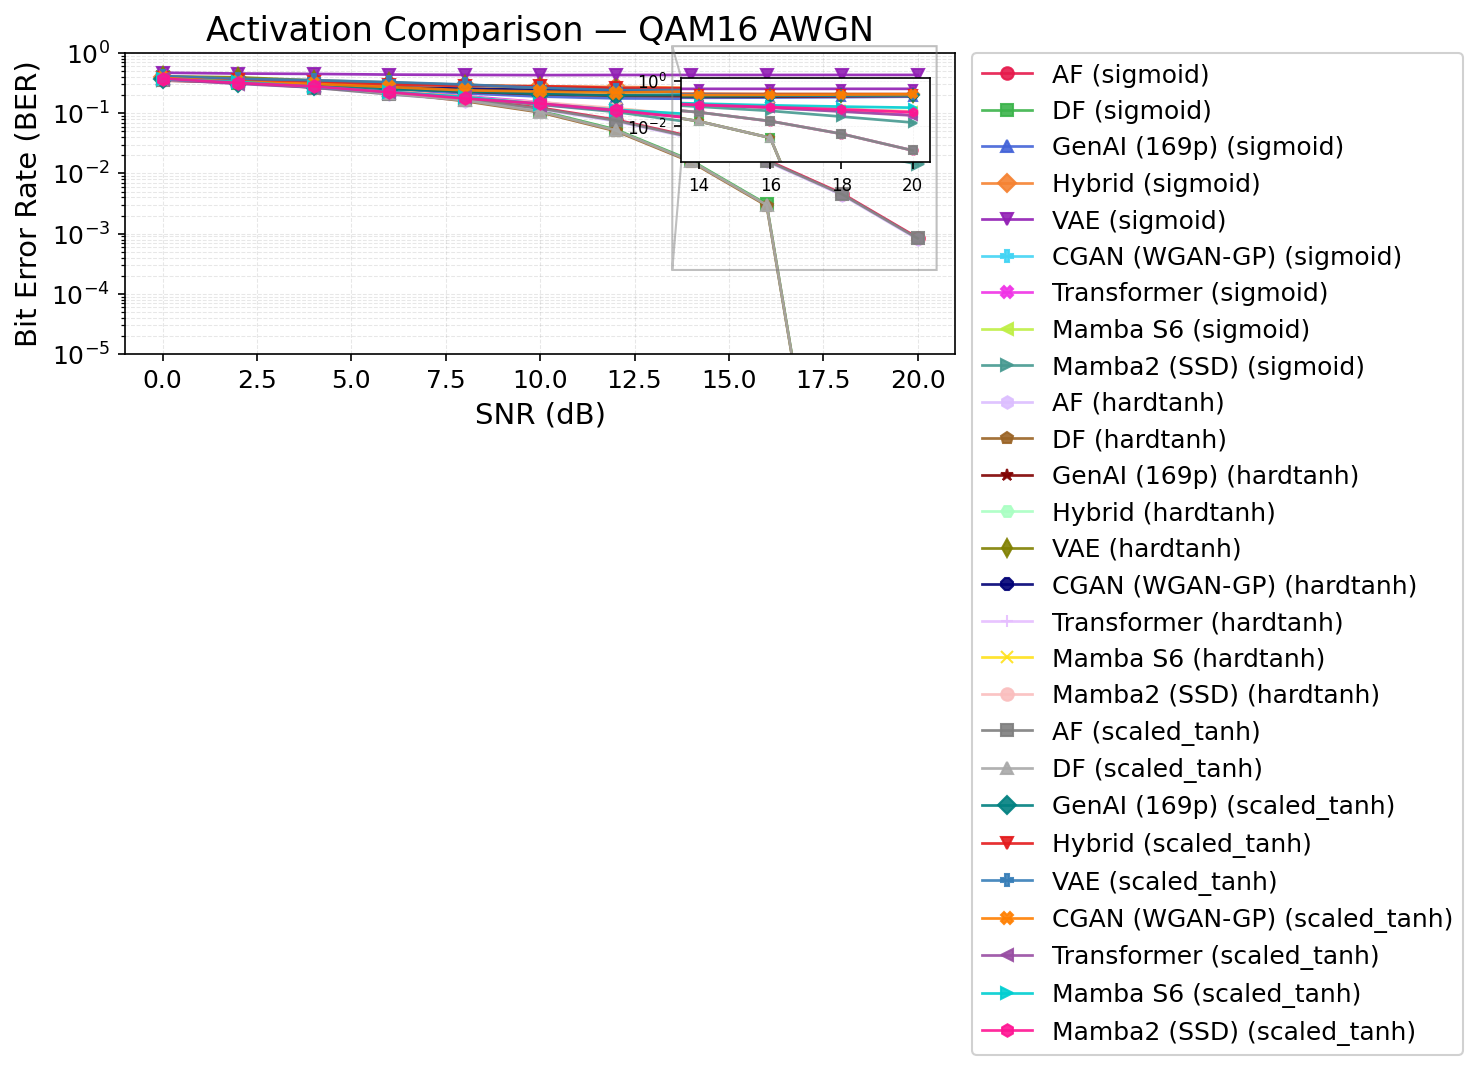
\includegraphics[width=\linewidth,height=0.45\textheight,keepaspectratio]{results/activation_comparison/qam16_activation_awgn.png}}
\caption{16-QAM constellation-aware activation comparison (AWGN). All three bounded activations eliminate the tanh BER floor from Section~\ref{sec:higher-order-modulation-scalability-constellation-aware-training}, with scaled tanh and hardtanh closely matched.}\label{fig:fig34}
\end{figure}

\begin{figure}[H]
\centering
\centering
\pandocbounded{
\includegraphics[width=\linewidth,height=0.45\textheight,keepaspectratio]{results/activation_comparison/qam16_activation_rayleigh.png}}
\caption{16-QAM constellation-aware activation comparison (Rayleigh fading). The BER floor elimination persists under fading. Sequence models benefit most from the constellation-aware bounds.}\label{fig:fig35}
\end{figure}

\begin{figure}[H]
\centering
\centering
\pandocbounded{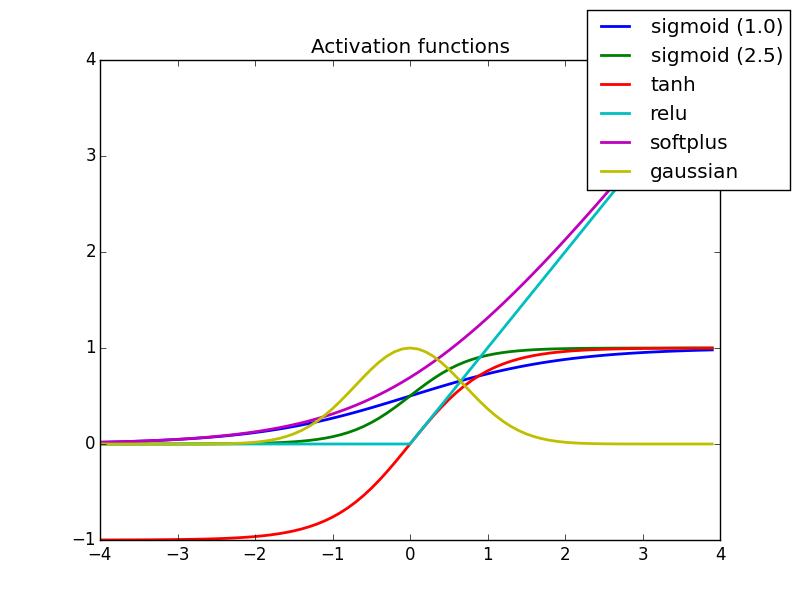
\includegraphics[width=\linewidth,height=0.45\textheight,keepaspectratio]{results/activation_comparison/various_activation_functions.png}}
\caption{Comparison of activation function shapes (left) and their derivatives (right) for \(A_{\max} = 0.9487\) (16-QAM). Hardtanh has a sharp transition at the clip bounds; sigmoid and scaled tanh provide smooth saturation with non-zero gradients throughout.}\label{fig:fig36}
\end{figure}

\section{Input Normalization and CSI Injection}\label{sec:input-normalization-and-csi-injection}

To evaluate the impact of explicit Channel State Information (CSI) injection and Input Layer Normalization across 48 distinct neural relay configurations (for 16-QAM and 16-PSK), an exhaustive hyperparameter sweep was conducted. Due to the volume of data, the full experimental methodology, BER vs. SNR charts, and detailed performance tables for all 48 variants have been relegated to \textbf{Appendix~\ref{chap:app-csi}}.

The key finding from this extensive experiment is a clear dichotomy: explicit CSI injection significantly improves performance for phase-only modulations (16-PSK) by resolving phase ambiguity, but actively degrades performance for amplitude-dependent modulations (16-QAM) by disrupting the delicate amplitude-decision boundaries. Input Layer Normalization proved universally beneficial.

\section{16-Class 2D Classification for QAM16}\label{sec:class-2d-classification-for-qam16}

\textbf{Goal:} Eliminate the structural BER floor imposed by per-axis I/Q splitting for 16-QAM by utilizing full 2D decision boundaries.

\textbf{Trials:} - \textbf{Topology:} SISO - \textbf{Modulation scheme:} 16-QAM - \textbf{Channel:} AWGN - \textbf{Equalizers:} None - \textbf{NN architecture:} Supervised (MLP), Generative (VAE), Sequence (Transformer, Mamba S6, Mamba-2 SSD) - \textbf{NN activation:} None (Softmax implicitly via Cross-Entropy loss) - \textbf{Special case:} 16-class joint 2D classification

\textbf{Conclusion:} Treating the relay as a joint 16-point classifier over the full 2D constellation space completely eliminates the structural 4-class BER floor. For the first time, neural variants (VAE, Transformer, MLP) matched classical DF performance at high SNR, achieving near-zero BER at 20 dB. This proves the previous BER floor was an artifact of I/Q splitting, not a fundamental limitation of neural relays.

\subsection{Results Tables}\label{sec:results-tables-5}

Table~\ref{tbl:table24} presents the BER at 20 dB for all variants alongside the classical AF and DF baselines.

\textit{[Detailed tabular results have been moved to Appendix~\ref{chap:app-tables}]}


\subsection{Results Figures}\label{sec:results-figures-6}

\begin{figure}[H]
\centering
\centering
\pandocbounded{
\includegraphics[width=\linewidth,height=0.45\textheight,keepaspectratio]{results/all_relays_16class/ber_all_relays_16class.png}}
\caption{16-QAM BER vs.~SNR for all relay variants (4-class and 16-class) on AWGN. The 4-class variants (dashed) plateau at BER ≈ 0.008 while the successfully trained 16-class variants (solid) continue decreasing, approaching and matching the DF baseline.}\label{fig:fig50}
\end{figure}

\begin{figure}[H]
\centering
\centering
\pandocbounded{
\includegraphics[width=\linewidth,height=0.45\textheight,keepaspectratio]{results/all_relays_16class/grouped_bar_16class.png}}
\caption{Grouped bar comparison of 4-class vs.~16-class BER at 20 dB for each architecture. The 16-class advantage is visible for MLP, VAE, Transformer, and Mamba S6. Failed variants (VAE 4-cls \textasciitilde0.50, CGAN 16-cls \textasciitilde0.50) are truncated.}\label{fig:fig51}
\end{figure}

\begin{figure}[H]
\centering
\centering
\pandocbounded{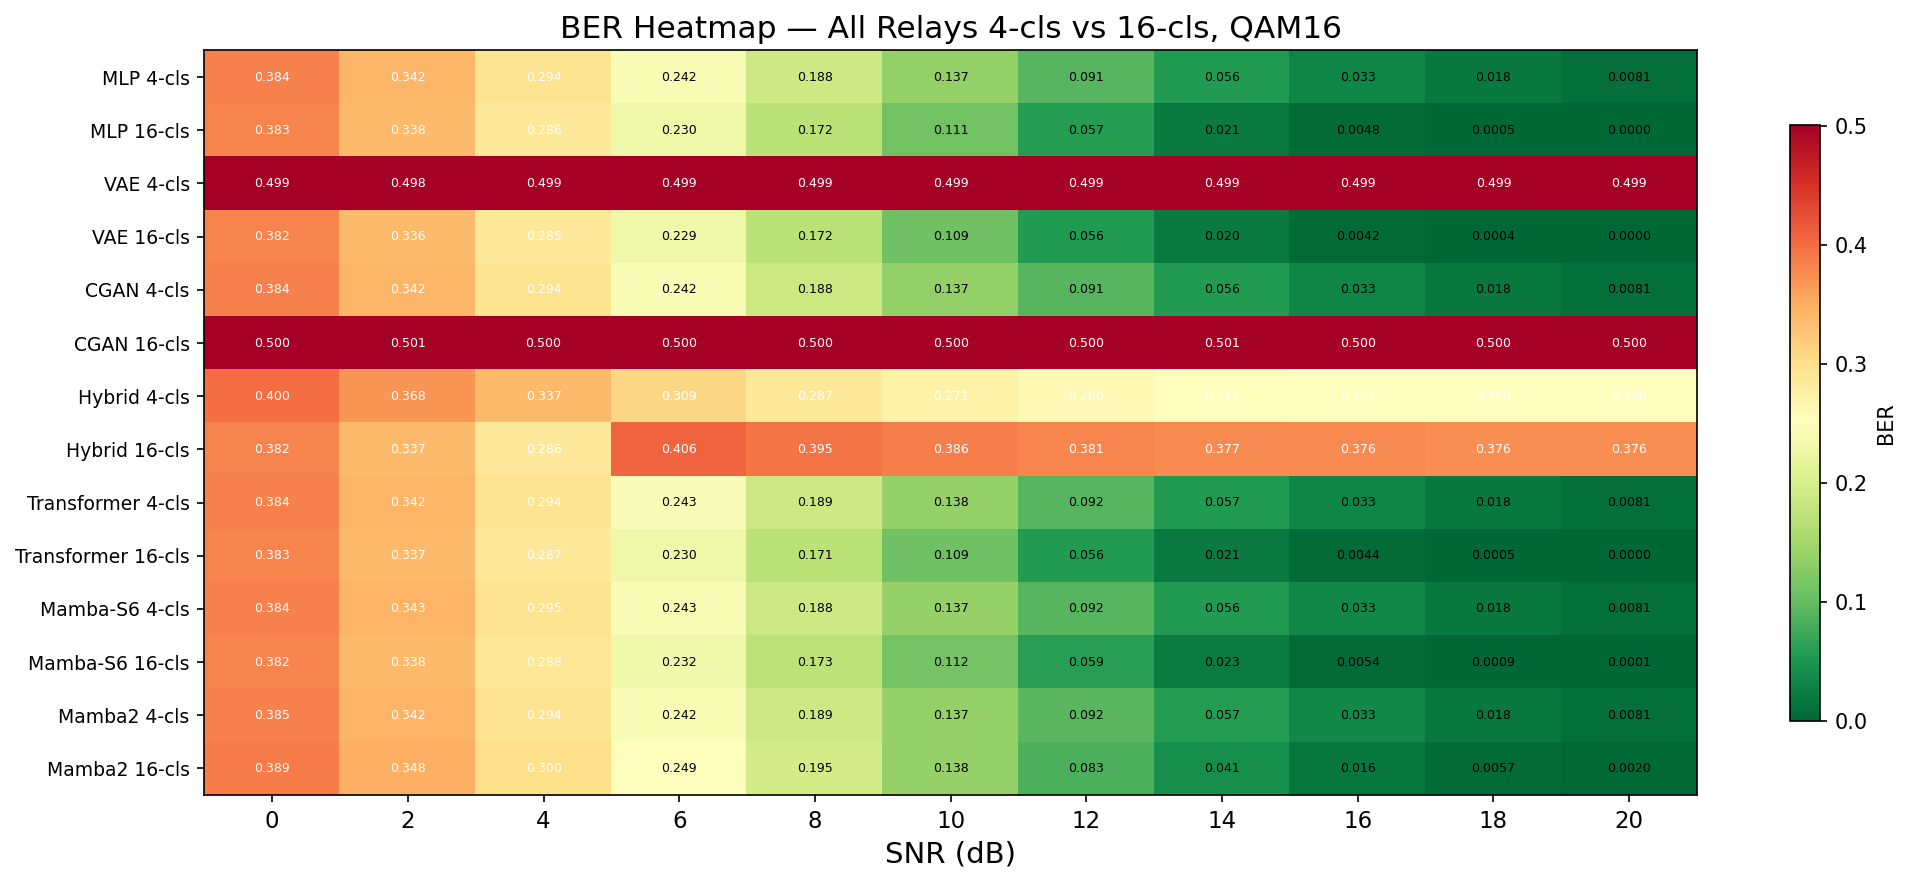
\includegraphics[width=\linewidth,height=0.45\textheight,keepaspectratio]{results/all_relays_16class/heatmap_all_relays_16class.png}}
\caption{Heatmap of BER across all relay variants and SNR points. The 16-class variants show a clear colour transition from high BER (warm) at low SNR to near-zero BER (cool) at high SNR, while 4-class variants remain warm at high SNR due to the structural floor.}\label{fig:fig52}
\end{figure}

\begin{figure}[H]
\centering
\centering
\pandocbounded{
\includegraphics[width=\linewidth,height=0.45\textheight,keepaspectratio]{results/all_relays_16class/top3_16class.png}}
\caption{Top-3 16-class relay variants compared against AF and DF. VAE 16-cls, Transformer 16-cls, and MLP 16-cls all match or approach DF performance across the full SNR range.}\label{fig:fig53}
\end{figure}

\section{End-to-End Joint Optimization}\label{sec:end-to-end-joint-optimization}

\textbf{Goal:} Compare the modular neural relay approach against a fully joint transmitter-receiver autoencoder.

\textbf{Trials:} - \textbf{Topology:} SISO - \textbf{Modulation scheme:} Learned latent space (M=16, power-constrained) - \textbf{Channel:} Rayleigh - \textbf{Equalizers:} ZF explicitly at the receiver - \textbf{NN architecture:} MLP Autoencoder (Encoder/Decoder) - \textbf{Special case:} End-to-End (E2E) optimization

\textbf{Conclusion:} The E2E autoencoder underperforms both the theoretical limits of classical 16-QAM and the modular two-hop DF relay across all SNR points (67-141\% higher BER). The network fails to discover a constellation geometry that surpasses the classical square grid under single-antenna Rayleigh fading, demonstrating that `black-box' deep learning is inefficient compared to modular designs that leverage classical signal processing algorithms for modulation and equalization.

\subsection{Results Figures}\label{sec:results-figures-7}

\begin{figure}[H]
\centering
\centering
\pandocbounded{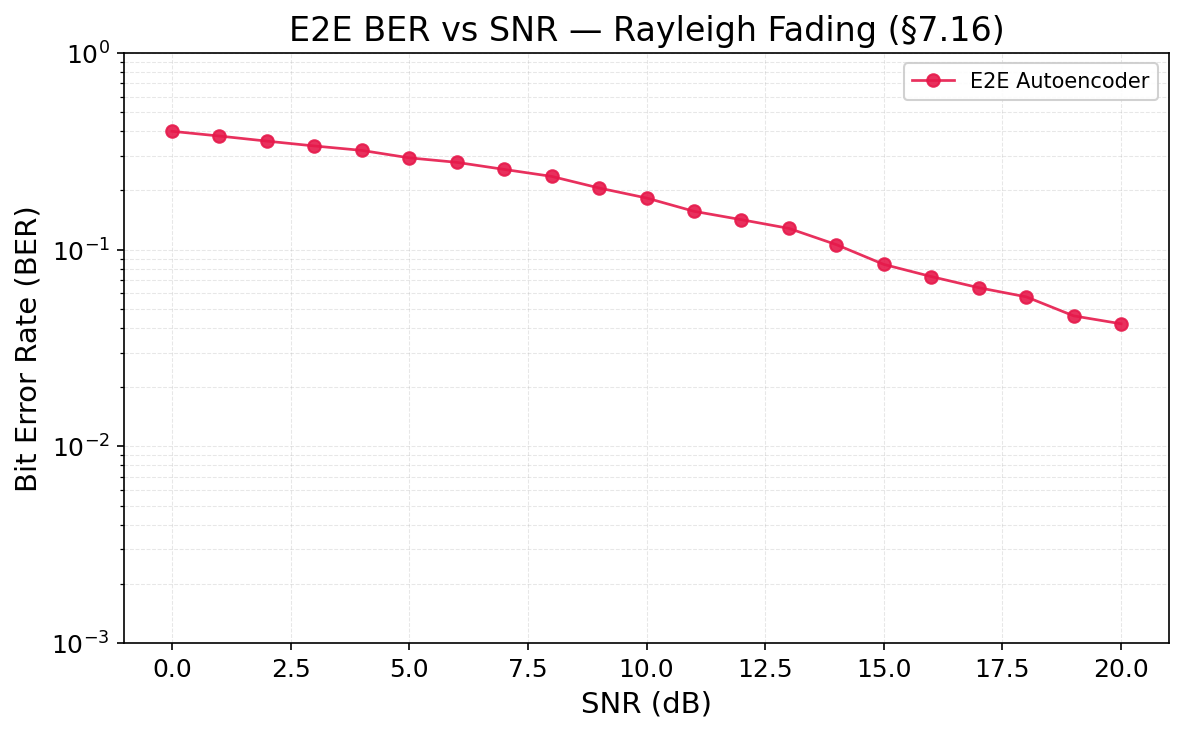
\includegraphics[width=\linewidth,height=0.45\textheight,keepaspectratio]{results/e2e/e2e_ber_comparison.png}}
\caption{BER vs.~SNR for E2E learned autoencoder compared to theoretical 16-QAM over Rayleigh fading. The E2E system underperforms the classical grid constellation across the full SNR range, with the gap widening at high SNR.}\label{fig:fig46}
\end{figure}

\begin{figure}[H]
\centering
\centering
\pandocbounded{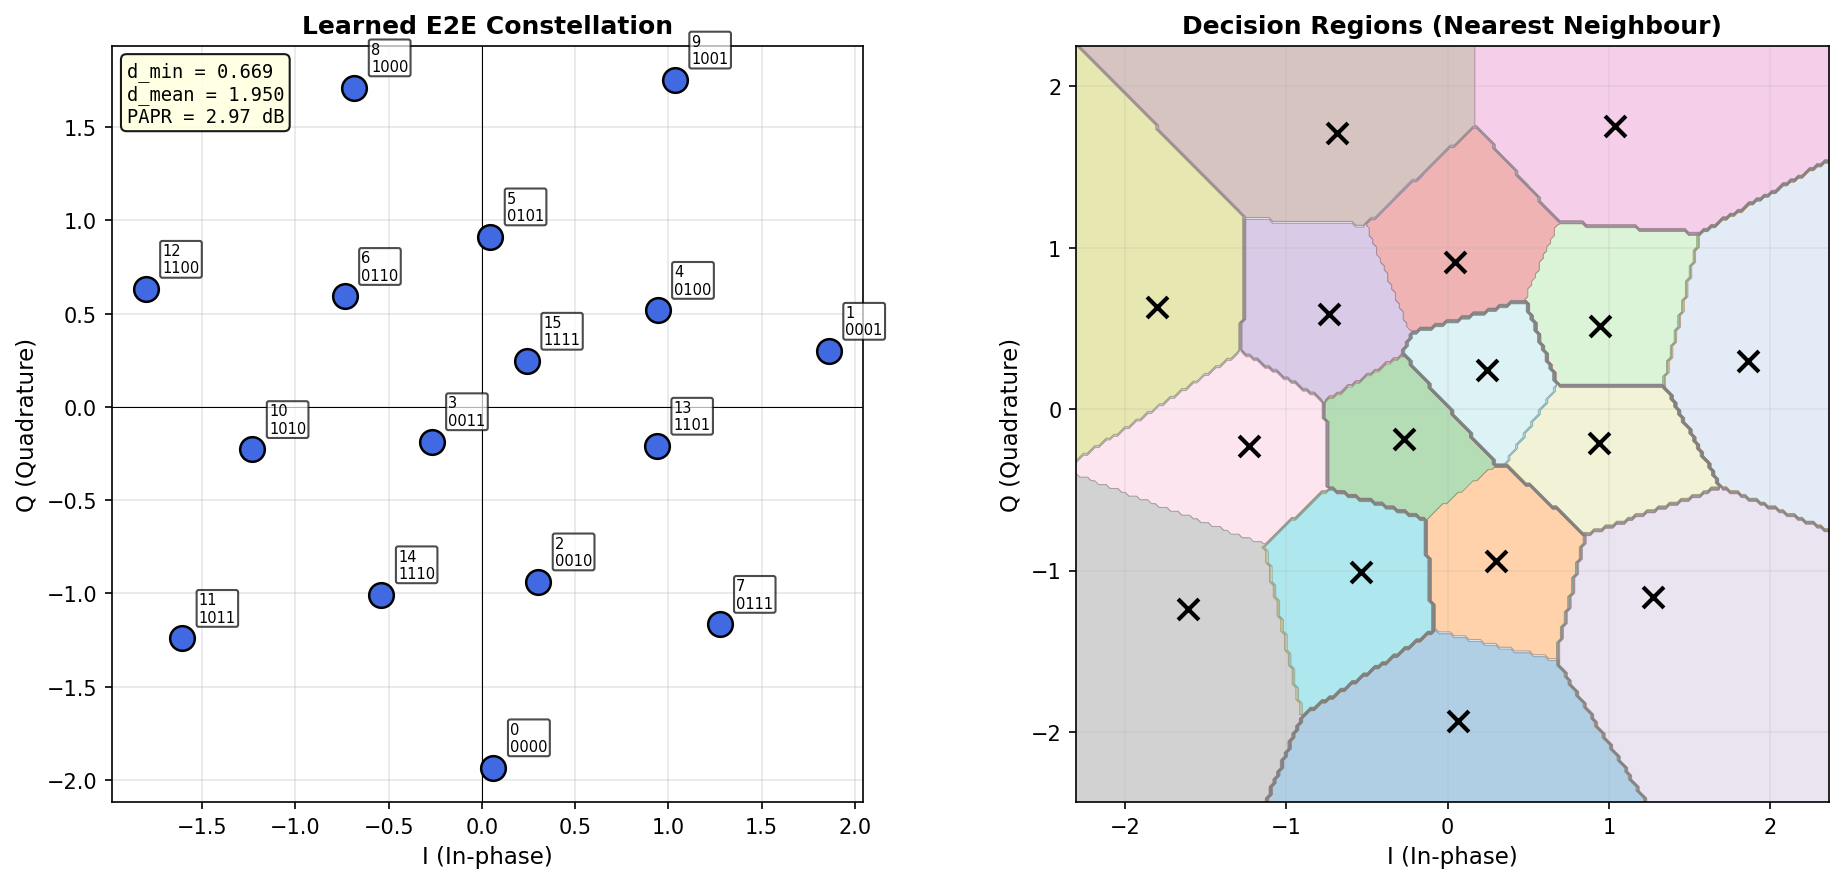
\includegraphics[width=\linewidth,height=0.45\textheight,keepaspectratio]{results/e2e/e2e_constellation.png}}
\caption{Learned 16-point constellation of the E2E autoencoder. The network discovers a non-rectangular geometry (resembling a hexagonal lattice or concentric APSK layout) that maximises minimum Euclidean distance under the average power constraint, unlike the classical \(4 \times 4\) square grid.}\label{fig:fig47}
\end{figure}

\begin{figure}[H]
\centering
\centering
\pandocbounded{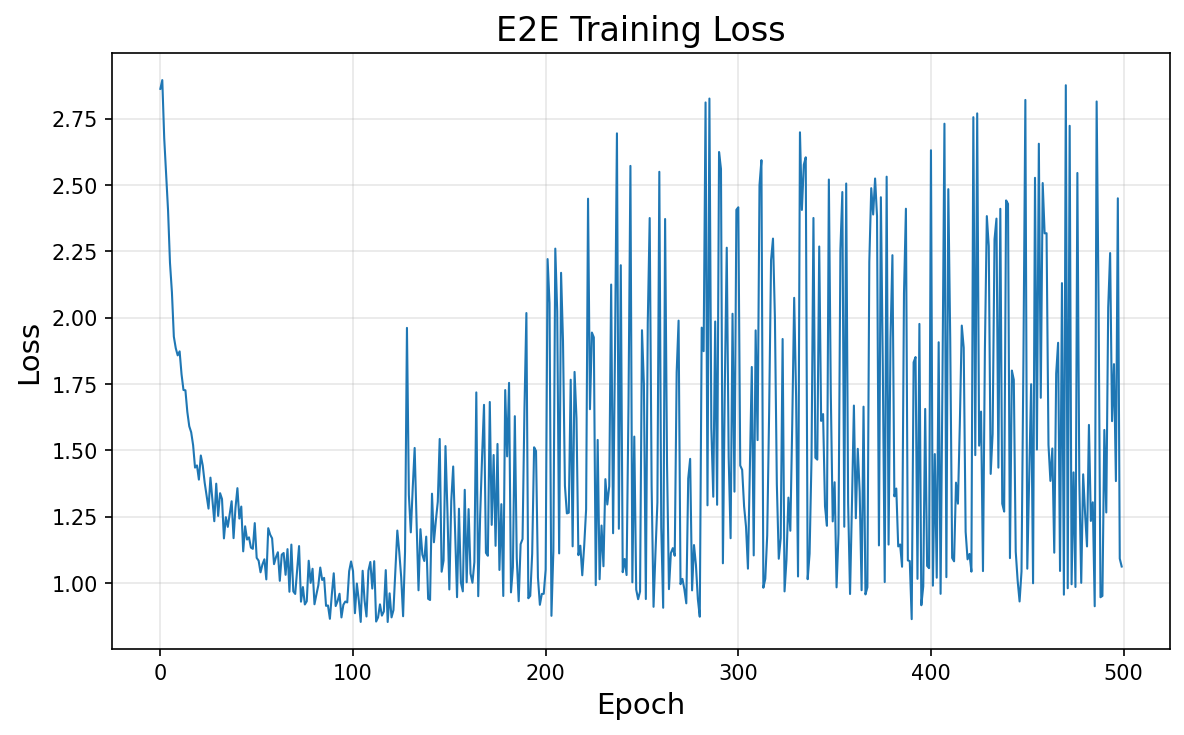
\includegraphics[width=\linewidth,height=0.45\textheight,keepaspectratio]{results/e2e/e2e_training_loss.png}}
\caption{Training loss (cross-entropy) convergence of the E2E autoencoder. The model converges within approximately 200 epochs.}\label{fig:fig48}
\end{figure}

\begin{figure}[H]
\centering
\centering
\pandocbounded{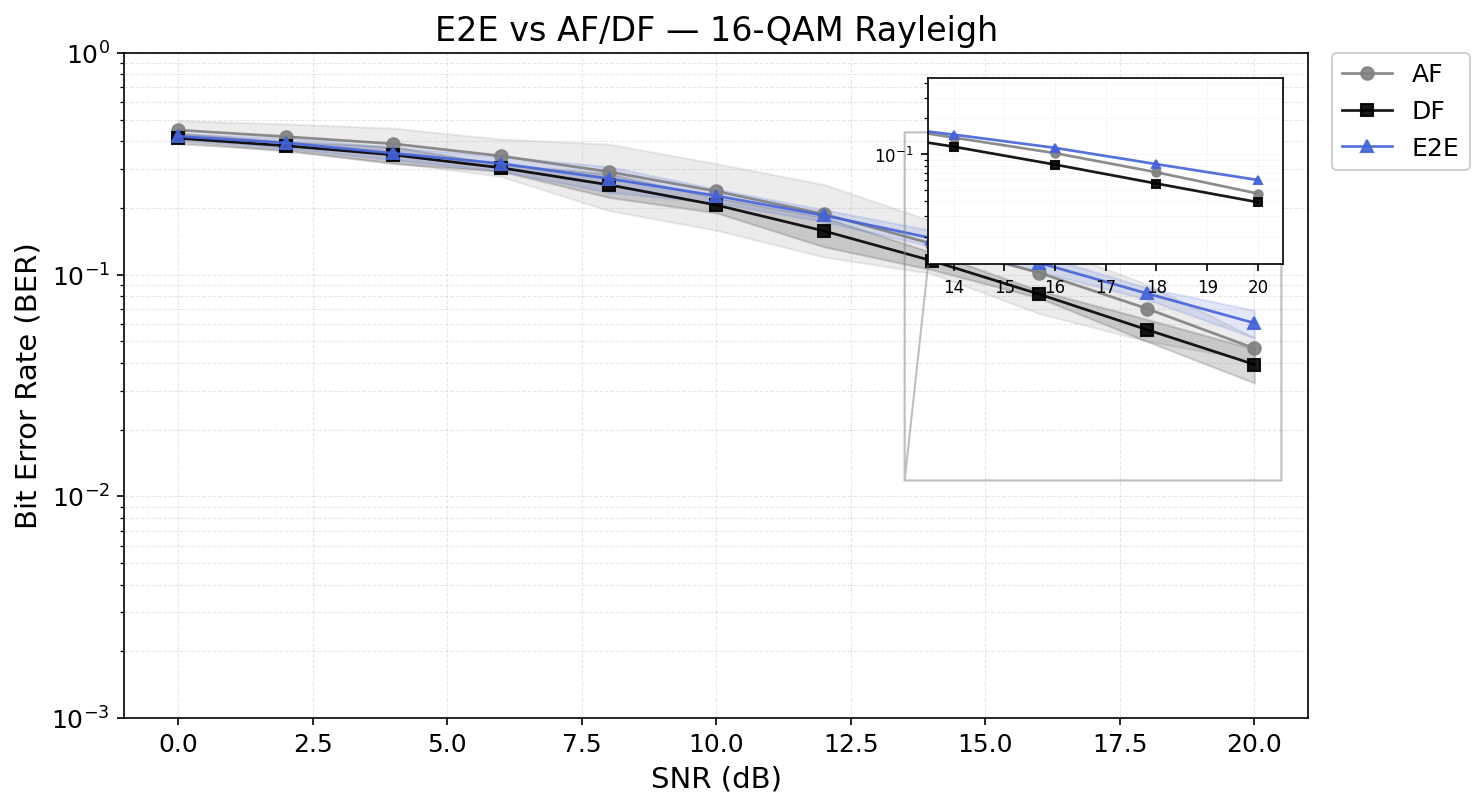
\includegraphics[width=\linewidth,height=0.45\textheight,keepaspectratio]{results/e2e/e2e_relay_comparison.png}}
\caption{Performance comparison of the E2E autoencoder against the modular relay-based approaches from this thesis. The E2E system does not achieve lower BER than the two-hop DF relay, highlighting the limitations of the E2E approach.}\label{fig:fig49}
\end{figure}

